\pgfdeclareplotmark{cross} {
\pgfpathmoveto{\pgfpoint{-0.3\pgfplotmarksize}{\pgfplotmarksize}}
\pgfpathlineto{\pgfpoint{+0.3\pgfplotmarksize}{\pgfplotmarksize}}
\pgfpathlineto{\pgfpoint{+0.3\pgfplotmarksize}{0.3\pgfplotmarksize}}
\pgfpathlineto{\pgfpoint{+1\pgfplotmarksize}{0.3\pgfplotmarksize}}
\pgfpathlineto{\pgfpoint{+1\pgfplotmarksize}{-0.3\pgfplotmarksize}}
\pgfpathlineto{\pgfpoint{+0.3\pgfplotmarksize}{-0.3\pgfplotmarksize}}
\pgfpathlineto{\pgfpoint{+0.3\pgfplotmarksize}{-1.\pgfplotmarksize}}
\pgfpathlineto{\pgfpoint{-0.3\pgfplotmarksize}{-1.\pgfplotmarksize}}
\pgfpathlineto{\pgfpoint{-0.3\pgfplotmarksize}{-0.3\pgfplotmarksize}}
\pgfpathlineto{\pgfpoint{-1.\pgfplotmarksize}{-0.3\pgfplotmarksize}}
\pgfpathlineto{\pgfpoint{-1.\pgfplotmarksize}{0.3\pgfplotmarksize}}
\pgfpathlineto{\pgfpoint{-0.3\pgfplotmarksize}{0.3\pgfplotmarksize}}
\pgfpathclose
\pgfusepathqstroke
}
\pgfdeclareplotmark{cross*} {
\pgfpathmoveto{\pgfpoint{-0.3\pgfplotmarksize}{\pgfplotmarksize}}
\pgfpathlineto{\pgfpoint{+0.3\pgfplotmarksize}{\pgfplotmarksize}}
\pgfpathlineto{\pgfpoint{+0.3\pgfplotmarksize}{0.3\pgfplotmarksize}}
\pgfpathlineto{\pgfpoint{+1\pgfplotmarksize}{0.3\pgfplotmarksize}}
\pgfpathlineto{\pgfpoint{+1\pgfplotmarksize}{-0.3\pgfplotmarksize}}
\pgfpathlineto{\pgfpoint{+0.3\pgfplotmarksize}{-0.3\pgfplotmarksize}}
\pgfpathlineto{\pgfpoint{+0.3\pgfplotmarksize}{-1.\pgfplotmarksize}}
\pgfpathlineto{\pgfpoint{-0.3\pgfplotmarksize}{-1.\pgfplotmarksize}}
\pgfpathlineto{\pgfpoint{-0.3\pgfplotmarksize}{-0.3\pgfplotmarksize}}
\pgfpathlineto{\pgfpoint{-1.\pgfplotmarksize}{-0.3\pgfplotmarksize}}
\pgfpathlineto{\pgfpoint{-1.\pgfplotmarksize}{0.3\pgfplotmarksize}}
\pgfpathlineto{\pgfpoint{-0.3\pgfplotmarksize}{0.3\pgfplotmarksize}}
\pgfpathclose
\pgfusepathqfillstroke
}
\pgfdeclareplotmark{newstar} {
\pgfpathmoveto{\pgfqpoint{0pt}{\pgfplotmarksize}}
\pgfpathlineto{\pgfqpointpolar{44}{0.5\pgfplotmarksize}}
\pgfpathlineto{\pgfqpointpolar{18}{\pgfplotmarksize}}
\pgfpathlineto{\pgfqpointpolar{-20}{0.5\pgfplotmarksize}}
\pgfpathlineto{\pgfqpointpolar{-54}{\pgfplotmarksize}}
\pgfpathlineto{\pgfqpointpolar{-90}{0.5\pgfplotmarksize}}
\pgfpathlineto{\pgfqpointpolar{234}{\pgfplotmarksize}}
\pgfpathlineto{\pgfqpointpolar{198}{0.5\pgfplotmarksize}}
\pgfpathlineto{\pgfqpointpolar{162}{\pgfplotmarksize}}
\pgfpathlineto{\pgfqpointpolar{134}{0.5\pgfplotmarksize}}
\pgfpathclose
\pgfusepathqstroke
}
\pgfdeclareplotmark{newstar*} {
\pgfpathmoveto{\pgfqpoint{0pt}{\pgfplotmarksize}}
\pgfpathlineto{\pgfqpointpolar{44}{0.5\pgfplotmarksize}}
\pgfpathlineto{\pgfqpointpolar{18}{\pgfplotmarksize}}
\pgfpathlineto{\pgfqpointpolar{-20}{0.5\pgfplotmarksize}}
\pgfpathlineto{\pgfqpointpolar{-54}{\pgfplotmarksize}}
\pgfpathlineto{\pgfqpointpolar{-90}{0.5\pgfplotmarksize}}
\pgfpathlineto{\pgfqpointpolar{234}{\pgfplotmarksize}}
\pgfpathlineto{\pgfqpointpolar{198}{0.5\pgfplotmarksize}}
\pgfpathlineto{\pgfqpointpolar{162}{\pgfplotmarksize}}
\pgfpathlineto{\pgfqpointpolar{134}{0.5\pgfplotmarksize}}
\pgfpathclose
\pgfusepathqfillstroke
}
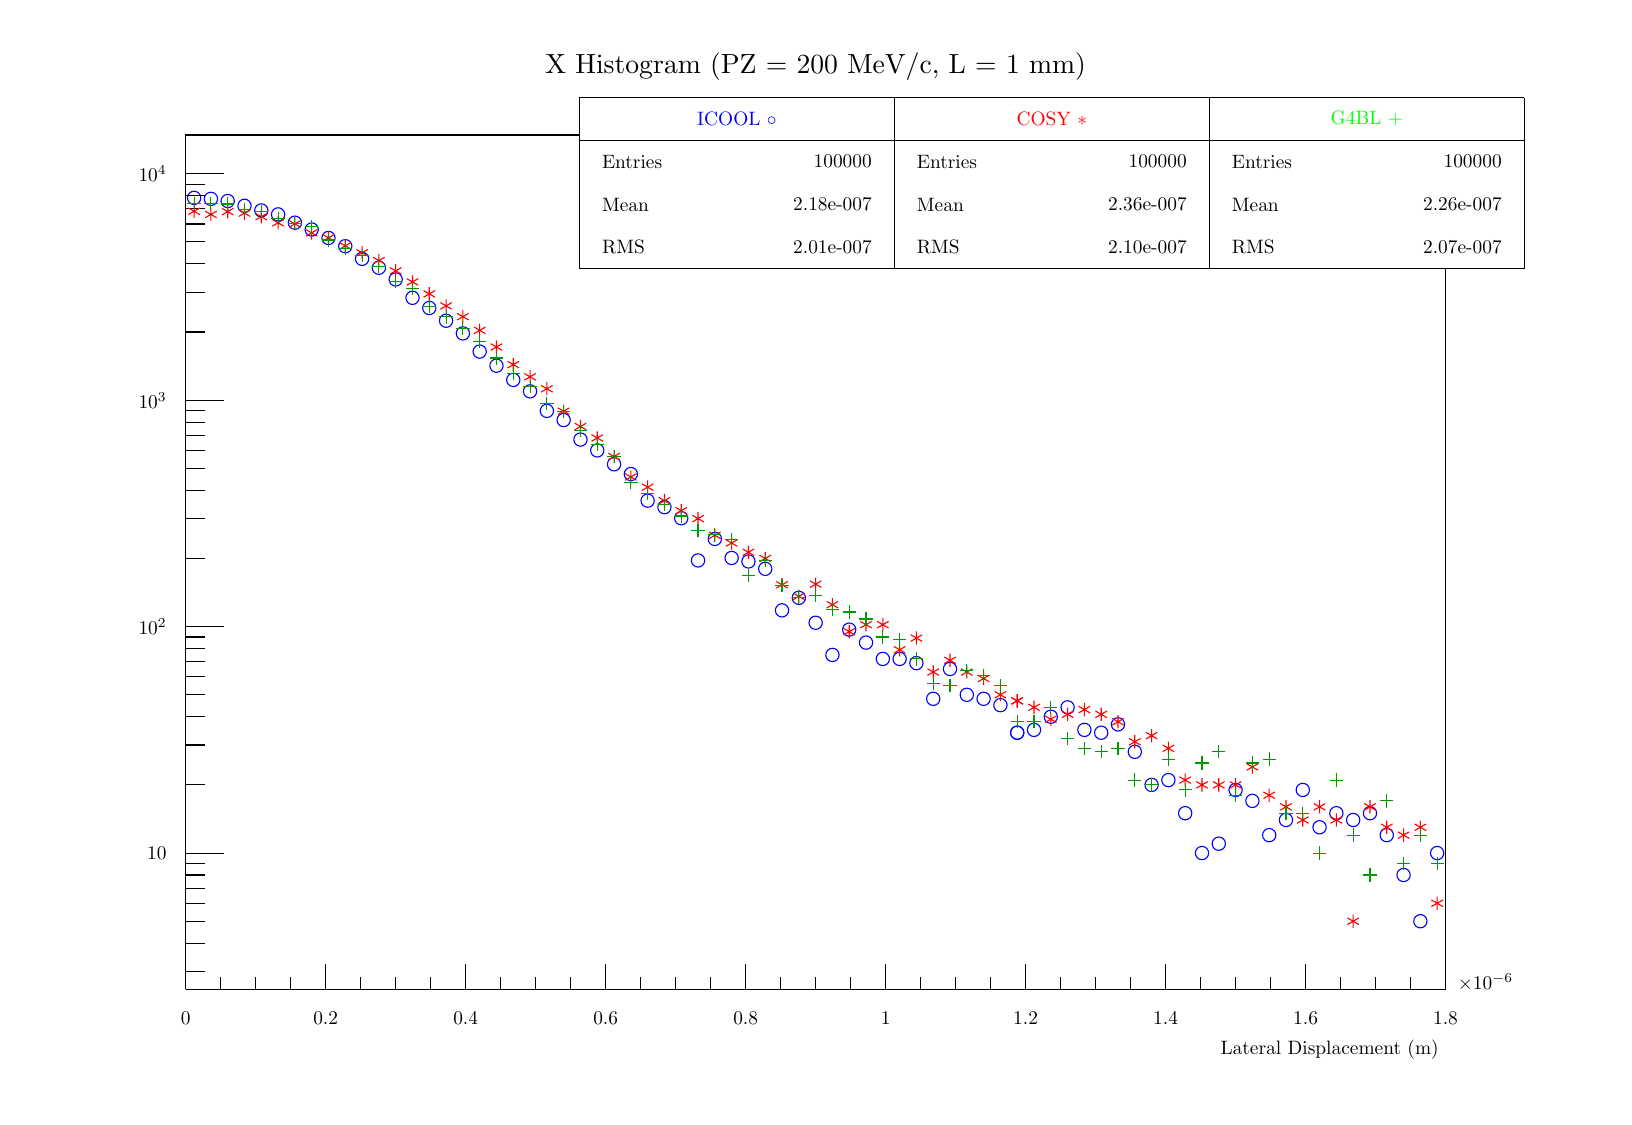
\begin{tikzpicture}
\definecolor{c}{rgb}{1,1,1};
\draw [color=c, fill=c] (0,0) rectangle (20,13.5632);
\draw [color=c, fill=c] (2,1.35632) rectangle (18,12.2069);
\definecolor{c}{rgb}{0,0,0};
\draw [c] (2,1.35632) -- (2,12.2069) -- (18,12.2069) -- (18,1.35632) -- (2,1.35632);
\definecolor{c}{rgb}{1,1,1};
\draw [color=c, fill=c] (2,1.35632) rectangle (18,12.2069);
\definecolor{c}{rgb}{0,0,0};
\draw [c] (2,1.35632) -- (2,12.2069) -- (18,12.2069) -- (18,1.35632) -- (2,1.35632);
\definecolor{c}{rgb}{0,0,1};
\foreach \P in
 {(2.10667,11.4087),(2.32,11.396),(2.53333,11.3685),(2.74667,11.3079),(2.96,11.249),(3.17333,11.1983),(3.38667,11.0937),(3.6,11.0072),(3.81333,10.8997),(4.02667,10.7946),(4.24,10.6344),(4.45333,10.5214),(4.66667,10.3726),(4.88,10.1395),(5.09333,10.01
),(5.30667,9.8483),(5.52,9.68748),(5.73333,9.45647),(5.94667,9.27733),(6.16,9.09691),(6.37333,8.95158),(6.58667,8.70362),(6.8,8.58694),(7.01333,8.3392),(7.22667,8.20138),(7.44,8.02505),(7.65333,7.90169),(7.86667,7.56338),(8.08,7.48093),(8.29333,7.339
83),(8.50667,6.80403),(8.72,7.07762),(8.93333,6.83549),(9.14667,6.79122),(9.36,6.69767),(9.57333,6.17028),(9.78667,6.32909),(10,6.01254),(10.2133,5.60426),(10.4267,5.92551),(10.64,5.76058),(10.8533,5.55327),(11.0667,5.55327),(11.28,5.50012),(11.4933,
5.04686),(11.7067,5.42553),(11.92,5.09785),(12.1333,5.04686),(12.3467,4.96626),(12.56,4.61617)}{\draw[mark options={color=c,fill=c},mark size=2.402402pt,mark=o] plot coordinates {\P};}
\foreach \P in
 {(12.56,4.61617),(12.7733,4.65238),(12.9867,4.81915),(13.2,4.93819),(13.4133,4.65238),(13.6267,4.61617),(13.84,4.72178),(14.0533,4.37368),(14.2667,3.95345),(14.48,4.01438),(14.6933,3.59414),(14.9067,3.08774),(15.12,3.20678),(15.3333,3.88938),(15.546
7,3.75047),(15.76,3.31545),(15.9733,3.50798),(16.1867,3.88938),(16.4,3.41542),(16.6133,3.59414),(16.8267,3.50798),(17.04,3.59414),(17.2533,3.31545),(17.4667,2.80904),(17.68,2.22203),(17.8933,3.08774)}{\draw[mark options={color=c,fill=c},mark
 size=2.402402pt,mark=o] plot coordinates {\P};}
\definecolor{c}{rgb}{1,1,1};
\draw [color=c, fill=c] (7,10.5115) rectangle (11,12.6816);
\definecolor{c}{rgb}{0,0,0};
\draw [c] (7,10.5115) -- (11,10.5115);
\draw [c] (11,10.5115) -- (11,12.6816);
\draw [c] (11,12.6816) -- (7,12.6816);
\draw [c] (7,12.6816) -- (7,10.5115);
\draw[color=blue](9,12.4103) node[scale=0.7, rotate=0]{ICOOL $\circ$};
\draw [c] (7,12.1391) -- (11,12.1391);
\draw [anchor= west] (7.2,11.8678) node[scale=0.7, rotate=0]{Entries };
\draw [anchor= east] (10.8,11.8678) node[scale=0.7, rotate=0]{ 100000};
\draw [anchor= west] (7.2,11.3253) node[scale=0.7, rotate=0]{Mean  };
\draw [anchor= east] (10.8,11.3253) node[scale=0.7, rotate=0]{ 2.18e-007};
\draw [anchor= west] (7.2,10.7828) node[scale=0.7, rotate=0]{RMS   };
\draw [anchor= east] (10.8,10.7828) node[scale=0.7, rotate=0]{ 2.01e-007};
\draw [c] (2,1.35632) -- (18,1.35632);
\draw [anchor= east] (18,0.596782) node[scale=0.7, rotate=0]{Lateral Displacement (m)};
\draw [c] (2,1.68184) -- (2,1.35632);
\draw [c] (2.44444,1.51908) -- (2.44444,1.35632);
\draw [c] (2.88889,1.51908) -- (2.88889,1.35632);
\draw [c] (3.33333,1.51908) -- (3.33333,1.35632);
\draw [c] (3.77778,1.68184) -- (3.77778,1.35632);
\draw [c] (4.22222,1.51908) -- (4.22222,1.35632);
\draw [c] (4.66667,1.51908) -- (4.66667,1.35632);
\draw [c] (5.11111,1.51908) -- (5.11111,1.35632);
\draw [c] (5.55556,1.68184) -- (5.55556,1.35632);
\draw [c] (6,1.51908) -- (6,1.35632);
\draw [c] (6.44444,1.51908) -- (6.44444,1.35632);
\draw [c] (6.88889,1.51908) -- (6.88889,1.35632);
\draw [c] (7.33333,1.68184) -- (7.33333,1.35632);
\draw [c] (7.77778,1.51908) -- (7.77778,1.35632);
\draw [c] (8.22222,1.51908) -- (8.22222,1.35632);
\draw [c] (8.66667,1.51908) -- (8.66667,1.35632);
\draw [c] (9.11111,1.68184) -- (9.11111,1.35632);
\draw [c] (9.55556,1.51908) -- (9.55556,1.35632);
\draw [c] (10,1.51908) -- (10,1.35632);
\draw [c] (10.4444,1.51908) -- (10.4444,1.35632);
\draw [c] (10.8889,1.68184) -- (10.8889,1.35632);
\draw [c] (11.3333,1.51908) -- (11.3333,1.35632);
\draw [c] (11.7778,1.51908) -- (11.7778,1.35632);
\draw [c] (12.2222,1.51908) -- (12.2222,1.35632);
\draw [c] (12.6667,1.68184) -- (12.6667,1.35632);
\draw [c] (13.1111,1.51908) -- (13.1111,1.35632);
\draw [c] (13.5556,1.51908) -- (13.5556,1.35632);
\draw [c] (14,1.51908) -- (14,1.35632);
\draw [c] (14.4444,1.68184) -- (14.4444,1.35632);
\draw [c] (14.8889,1.51908) -- (14.8889,1.35632);
\draw [c] (15.3333,1.51908) -- (15.3333,1.35632);
\draw [c] (15.7778,1.51908) -- (15.7778,1.35632);
\draw [c] (16.2222,1.68184) -- (16.2222,1.35632);
\draw [c] (16.6667,1.51908) -- (16.6667,1.35632);
\draw [c] (17.1111,1.51908) -- (17.1111,1.35632);
\draw [c] (17.5556,1.51908) -- (17.5556,1.35632);
\draw [c] (18,1.68184) -- (18,1.35632);
\draw [anchor=base] (2,0.908736) node[scale=0.7, rotate=0]{0};
\draw [anchor=base] (3.77778,0.908736) node[scale=0.7, rotate=0]{0.2};
\draw [anchor=base] (5.55556,0.908736) node[scale=0.7, rotate=0]{0.4};
\draw [anchor=base] (7.33333,0.908736) node[scale=0.7, rotate=0]{0.6};
\draw [anchor=base] (9.11111,0.908736) node[scale=0.7, rotate=0]{0.8};
\draw [anchor=base] (10.8889,0.908736) node[scale=0.7, rotate=0]{1};
\draw [anchor=base] (12.6667,0.908736) node[scale=0.7, rotate=0]{1.2};
\draw [anchor=base] (14.4444,0.908736) node[scale=0.7, rotate=0]{1.4};
\draw [anchor=base] (16.2222,0.908736) node[scale=0.7, rotate=0]{1.6};
\draw [anchor=base] (18,0.908736) node[scale=0.7, rotate=0]{1.8};
\draw [anchor=base west] (18.07,1.35632) node[scale=0.7, rotate=0]{$\times10^{-6}$};
\draw [c] (2,1.35632) -- (2,12.2069);
\draw [c] (2.24,1.58403) -- (2,1.58403);
\draw [c] (2.24,1.94333) -- (2,1.94333);
\draw [c] (2.24,2.22203) -- (2,2.22203);
\draw [c] (2.24,2.44974) -- (2,2.44974);
\draw [c] (2.24,2.64226) -- (2,2.64226);
\draw [c] (2.24,2.80904) -- (2,2.80904);
\draw [c] (2.24,2.95614) -- (2,2.95614);
\draw [c] (2.48,3.08774) -- (2,3.08774);
\draw [anchor= east] (1.844,3.08774) node[scale=0.7, rotate=0]{10};
\draw [c] (2.24,3.95344) -- (2,3.95344);
\draw [c] (2.24,4.45985) -- (2,4.45985);
\draw [c] (2.24,4.81915) -- (2,4.81915);
\draw [c] (2.24,5.09785) -- (2,5.09785);
\draw [c] (2.24,5.32556) -- (2,5.32556);
\draw [c] (2.24,5.51809) -- (2,5.51809);
\draw [c] (2.24,5.68486) -- (2,5.68486);
\draw [c] (2.24,5.83196) -- (2,5.83196);
\draw [c] (2.48,5.96356) -- (2,5.96356);
\draw [anchor= east] (1.844,5.96356) node[scale=0.7, rotate=0]{$10^{2}$};
\draw [c] (2.24,6.82926) -- (2,6.82926);
\draw [c] (2.24,7.33567) -- (2,7.33567);
\draw [c] (2.24,7.69497) -- (2,7.69497);
\draw [c] (2.24,7.97367) -- (2,7.97367);
\draw [c] (2.24,8.20138) -- (2,8.20138);
\draw [c] (2.24,8.3939) -- (2,8.3939);
\draw [c] (2.24,8.56068) -- (2,8.56068);
\draw [c] (2.24,8.70778) -- (2,8.70778);
\draw [c] (2.48,8.83938) -- (2,8.83938);
\draw [anchor= east] (1.844,8.83938) node[scale=0.7, rotate=0]{$10^{3}$};
\draw [c] (2.24,9.70508) -- (2,9.70508);
\draw [c] (2.24,10.2115) -- (2,10.2115);
\draw [c] (2.24,10.5708) -- (2,10.5708);
\draw [c] (2.24,10.8495) -- (2,10.8495);
\draw [c] (2.24,11.0772) -- (2,11.0772);
\draw [c] (2.24,11.2697) -- (2,11.2697);
\draw [c] (2.24,11.4365) -- (2,11.4365);
\draw [c] (2.24,11.5836) -- (2,11.5836);
\draw [c] (2.48,11.7152) -- (2,11.7152);
\draw [anchor= east] (1.844,11.7152) node[scale=0.7, rotate=0]{$10^{4}$};
\definecolor{c}{rgb}{1,1,1};
\draw [color=c, fill=c] (7,10.5115) rectangle (11,12.6816);
\definecolor{c}{rgb}{0,0,0};
\draw [c] (7,10.5115) -- (11,10.5115);
\draw [c] (11,10.5115) -- (11,12.6816);
\draw [c] (11,12.6816) -- (7,12.6816);
\draw [c] (7,12.6816) -- (7,10.5115);
\draw[color=blue](9,12.4103) node[scale=0.7, rotate=0]{ICOOL $\circ$};
\draw [c] (7,12.1391) -- (11,12.1391);
\draw [anchor= west] (7.2,11.8678) node[scale=0.7, rotate=0]{Entries };
\draw [anchor= east] (10.8,11.8678) node[scale=0.7, rotate=0]{ 100000};
\draw [anchor= west] (7.2,11.3253) node[scale=0.7, rotate=0]{Mean  };
\draw [anchor= east] (10.8,11.3253) node[scale=0.7, rotate=0]{ 2.18e-007};
\draw [anchor= west] (7.2,10.7828) node[scale=0.7, rotate=0]{RMS   };
\draw [anchor= east] (10.8,10.7828) node[scale=0.7, rotate=0]{ 2.01e-007};
\draw (10,13.0816) node[scale=1, rotate=0]{X Histogram (PZ = 200 MeV/c, L = 1 mm)};
\definecolor{c}{rgb}{1,0,0};
\foreach \P in
 {(2.10667,11.2381),(2.32,11.1979),(2.53333,11.2339),(2.74667,11.2145),(2.96,11.1691),(3.17333,11.0923),(3.38667,11.0787),(3.6,10.9637),(3.81333,10.9011),(4.02667,10.7993),(4.24,10.7121),(4.45333,10.6125),(4.66667,10.4812),(4.88,10.3407),(5.09333,10.
1892),(5.30667,10.0366),(5.52,9.90011),(5.73333,9.72614),(5.94667,9.51453),(6.16,9.29132),(6.37333,9.13593),(6.58667,8.98426),(6.8,8.69943),(7.01333,8.50481),(7.22667,8.35954),(7.44,8.1241),(7.65333,7.86409),(7.86667,7.73492),(8.08,7.56338),(8.29333,
7.43564),(8.50667,7.33567),(8.72,7.12286),(8.93333,7.02535),(9.14667,6.90792),(9.36,6.82926),(9.57333,6.4947),(9.78667,6.34759),(10,6.50283),(10.2133,6.24225),(10.4267,5.89949),(10.64,5.98829),(10.8533,5.98829),(11.0667,5.66915),(11.28,5.81801),(11.4
933,5.3865),(11.7067,5.5358),(11.92,5.3865),(12.1333,5.30457),(12.3467,5.09785),(12.56,5.02057)}{\draw[mark options={color=c,fill=c},mark size=2.402402pt,mark=asterisk] plot coordinates {\P};}
\foreach \P in
 {(12.56,5.02057),(12.7733,4.93819),(12.9867,4.78753),(13.2,4.84999),(13.4133,4.90948),(13.6267,4.84999),(13.84,4.75509),(14.0533,4.5008),(14.2667,4.57889),(14.48,4.41751),(14.6933,4.01438),(14.9067,3.95345),(15.12,3.95345),(15.3333,3.95345),(15.5467
,4.18116),(15.76,3.82186),(15.9733,3.67475),(16.1867,3.50798),(16.4,3.67475),(16.6133,3.50798),(16.8267,2.22203),(17.04,3.67475),(17.2533,3.41542),(17.4667,3.31545),(17.68,3.41542),(17.8933,2.44974)}{\draw[mark options={color=c,fill=c},mark
 size=2.402402pt,mark=asterisk] plot coordinates {\P};}
\definecolor{c}{rgb}{1,1,1};
\draw [color=c, fill=c] (11,10.5115) rectangle (15,12.6816);
\definecolor{c}{rgb}{0,0,0};
\draw [c] (11,10.5115) -- (15,10.5115);
\draw [c] (15,10.5115) -- (15,12.6816);
\draw [c] (15,12.6816) -- (11,12.6816);
\draw [c] (11,12.6816) -- (11,10.5115);
\draw [color=red](13,12.4103) node[scale=0.7, rotate=0]{COSY $*$};
\draw [c] (11,12.1391) -- (15,12.1391);
\draw [anchor= west] (11.2,11.8678) node[scale=0.7, rotate=0]{Entries };
\draw [anchor= east] (14.8,11.8678) node[scale=0.7, rotate=0]{ 100000};
\draw [anchor= west] (11.2,11.3253) node[scale=0.7, rotate=0]{Mean  };
\draw [anchor= east] (14.8,11.3253) node[scale=0.7, rotate=0]{ 2.36e-007};
\draw [anchor= west] (11.2,10.7828) node[scale=0.7, rotate=0]{RMS   };
\draw [anchor= east] (14.8,10.7828) node[scale=0.7, rotate=0]{ 2.10e-007};
\definecolor{c}{rgb}{1,1,1};
\draw [color=c, fill=c] (11,10.5115) rectangle (15,12.6816);
\definecolor{c}{rgb}{0,0,0};
\draw [c] (11,10.5115) -- (15,10.5115);
\draw [c] (15,10.5115) -- (15,12.6816);
\draw [c] (15,12.6816) -- (11,12.6816);
\draw [c] (11,12.6816) -- (11,10.5115);
\draw [color=red](13,12.4103) node[scale=0.7, rotate=0]{COSY $*$};
\draw [c] (11,12.1391) -- (15,12.1391);
\draw [anchor= west] (11.2,11.8678) node[scale=0.7, rotate=0]{Entries };
\draw [anchor= east] (14.8,11.8678) node[scale=0.7, rotate=0]{ 100000};
\draw [anchor= west] (11.2,11.3253) node[scale=0.7, rotate=0]{Mean  };
\draw [anchor= east] (14.8,11.3253) node[scale=0.7, rotate=0]{ 2.36e-007};
\draw [anchor= west] (11.2,10.7828) node[scale=0.7, rotate=0]{RMS   };
\draw [anchor= east] (14.8,10.7828) node[scale=0.7, rotate=0]{ 2.10e-007};
\definecolor{c}{rgb}{0,0.6,0};
\foreach \P in
 {(2.10667,11.3386),(2.32,11.3364),(2.53333,11.3313),(2.74667,11.2563),(2.96,11.235),(3.17333,11.151),(3.38667,11.0807),(3.6,11.04),(3.81333,10.8732),(4.02667,10.7698),(4.24,10.6747),(4.45333,10.5411),(4.66667,10.3497),(4.88,10.2577),(5.09333,10.0332
),(5.30667,9.8969),(5.52,9.75407),(5.73333,9.58455),(5.94667,9.37459),(6.16,9.18139),(6.37333,9.01502),(6.58667,8.80133),(6.8,8.69243),(7.01333,8.45314),(7.22667,8.27415),(7.44,8.11966),(7.65333,7.79398),(7.86667,7.65048),(8.08,7.51023),(8.29333,7.36
854),(8.50667,7.18544),(8.72,7.12779),(8.93333,7.06734),(9.14667,6.61151),(9.36,6.80403),(9.57333,6.48651),(9.78667,6.33837),(10,6.35674),(10.2133,6.18082),(10.4267,6.14893),(10.64,6.05968),(10.8533,5.83197),(11.0667,5.8039),(11.28,5.55327),(11.4933,
5.23939),(11.7067,5.21689),(11.92,5.40617),(12.1333,5.3462),(12.3467,5.21689),(12.56,4.75509)}{\draw[mark options={color=c,fill=c},mark size=2.402402pt,mark=+] plot coordinates {\P};}
\foreach \P in
 {(12.56,4.75509),(12.7733,4.75509),(12.9867,4.93819),(13.2,4.54046),(13.4133,4.41751),(13.6267,4.37368),(13.84,4.41751),(14.0533,4.01438),(14.2667,3.95345),(14.48,4.28113),(14.6933,3.88938),(14.9067,4.23214),(15.12,4.37368),(15.3333,3.82186),(15.546
7,4.23214),(15.76,4.28113),(15.9733,3.59414),(16.1867,3.59414),(16.4,3.08774),(16.6133,4.01438),(16.8267,3.31545),(17.04,2.80904),(17.2533,3.75047),(17.4667,2.95615),(17.68,3.31545),(17.8933,2.95615)}{\draw[mark options={color=c,fill=c},mark
 size=2.402402pt,mark=+] plot coordinates {\P};}
\definecolor{c}{rgb}{1,1,1};
\draw [color=c, fill=c] (15,10.5115) rectangle (19,12.6816);
\definecolor{c}{rgb}{0,0,0};
\draw [c] (15,10.5115) -- (19,10.5115);
\draw [c] (19,10.5115) -- (19,12.6816);
\draw [c] (19,12.6816) -- (15,12.6816);
\draw [c] (15,12.6816) -- (15,10.5115);
\draw [color=green](17,12.4103) node[scale=0.7, rotate=0]{G4BL $+$};
\draw [c] (15,12.1391) -- (19,12.1391);
\draw [anchor= west] (15.2,11.8678) node[scale=0.7, rotate=0]{Entries };
\draw [anchor= east] (18.8,11.8678) node[scale=0.7, rotate=0]{ 100000};
\draw [anchor= west] (15.2,11.3253) node[scale=0.7, rotate=0]{Mean  };
\draw [anchor= east] (18.8,11.3253) node[scale=0.7, rotate=0]{ 2.26e-007};
\draw [anchor= west] (15.2,10.7828) node[scale=0.7, rotate=0]{RMS   };
\draw [anchor= east] (18.8,10.7828) node[scale=0.7, rotate=0]{ 2.07e-007};
\definecolor{c}{rgb}{1,1,1};
\draw [color=c, fill=c] (15,10.5115) rectangle (19,12.6816);
\definecolor{c}{rgb}{0,0,0};
\draw [c] (15,10.5115) -- (19,10.5115);
\draw [c] (19,10.5115) -- (19,12.6816);
\draw [c] (19,12.6816) -- (15,12.6816);
\draw [c] (15,12.6816) -- (15,10.5115);
\draw [color=green](17,12.4103) node[scale=0.7, rotate=0]{G4BL $+$};
\draw [c] (15,12.1391) -- (19,12.1391);
\draw [anchor= west] (15.2,11.8678) node[scale=0.7, rotate=0]{Entries };
\draw [anchor= east] (18.8,11.8678) node[scale=0.7, rotate=0]{ 100000};
\draw [anchor= west] (15.2,11.3253) node[scale=0.7, rotate=0]{Mean  };
\draw [anchor= east] (18.8,11.3253) node[scale=0.7, rotate=0]{ 2.26e-007};
\draw [anchor= west] (15.2,10.7828) node[scale=0.7, rotate=0]{RMS   };
\draw [anchor= east] (18.8,10.7828) node[scale=0.7, rotate=0]{ 2.07e-007};
\end{tikzpicture}
